\chapter{Game Rules and Mechanics}
\label{chapter02}

For the purposes of this thesis we'll only stick to turn-based gameplay. We
still wanted our game to be general enough so that a wide variety of
playstyles can be represented within the game rules.

Two teams fight on a hexagonal map (\emph{arena}) of small size (radius of
5--10 hexes, see \hyperref[fig:arena]{Figure 2.1}). Each team consists of a small number of player controller
characters (\emph{mages} for short), and each mage has a small number of
\emph{abilities}, \emph{health}, and \emph{action points}. Players take turns, during
which each player has control over one of his mages. The player can issue
commands to move around the arena and use abilities. Both movement and ability
usage costs action points, which are restored at the end of the turn.  Moving
one hex costs one action point. The cost of using an ability varies, and is one
of the parameters that we optimize for when looking for a balanaced game. An
ability can also have a \emph{cooldown}, which prevents repeated usage for a
given number of rounds. Note that the cooldown can be zero, which means the
ability can be used multiple times per turn

Abilities can do direct damage to an enemy mage, apply a \emph{debuff} (causing
damage and decreasing action points over time), and create an area of effect
(\emph{AOE}) debuff that spans multiple hexes in the arena. Both the debuffs and
AOEs are applied at the end of each round. Both debuffs and AOEs also have a lifetime,
which specifies how many rounds the effect lasts.

There is also an important distinction between a \emph{turn} and a \emph{round}.
A turn means playing all the actions a single mage can do with his action points,
and ends when the player decides he is finished playing with that one single character.
A round ends when all of the characters have played their turn, and it is at that point
when debuffs, AOEs, cooldowns and action points are re-calculated (see below).

The motivation for having cooldowns is that it allows us to generate powerful
abilities that don't necessarily take up the whole turn of the player by costing
a lot of action points. If the ability is cheap, but has a large cooldown, it can
serve a strategic purpose, as the player might want to prepare his position in order
to use the ability when the cooldown wears off. AOE abilities also improve positional
gameplay, as they can be used to force the enemy player to move out of position.

\begin{figure}[h]
	\centering
	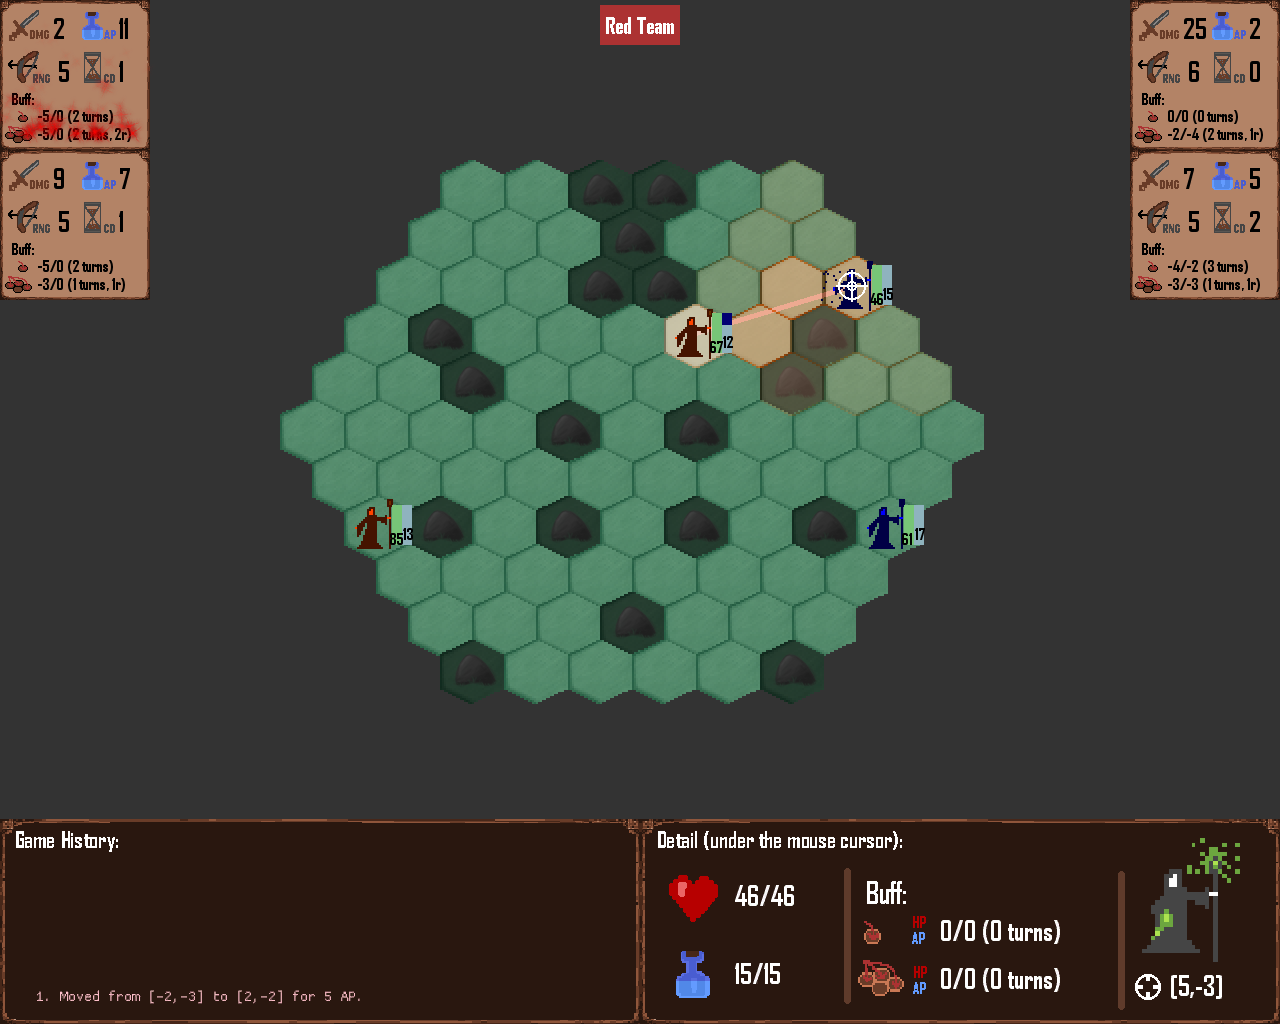
\includegraphics[width=0.95\textwidth]{img/arena.png}
	\caption{User interface of the HexMage game, featuring a 2v2 game. The red player currently has a spell selected and is targeting one of the blue player's mages.}	
	\label{fig:arena}
\end{figure}


\section{Simulator}

Part of our game is a simulator that can be used as a library and encapsulates
all of the game rules and mechanics. This is then used by both the AI and the
PCG algorithm and can thus be run separately from the main game. The game is
internally represented by a \emph{state} object, and all of the possible player
actions are encapsulated by an \emph{action} object.  Playing the game through
the library then simply becomes a matter of applying a state transition
function $f: (\text{state}, \text{action}) \rightarrow \text{state}$. The
simulator also verifies that no invalid actions are applied through a thorough
list of invariant checks. These are automatically turned off in a release build
to make the simulator run as fast as possible.

The simulator is also built to be high performance and can easily run hundreds
of thousands to millions of actions per second on a consumer-grade PC. 
The state object is split into two parts, one that handles the
general immutable information that doesn't change as the game progresses (i.e.
max hitpoints, ability definitions, etc.), and one that handles all of the
mutable data, such as current hitpoints, current positions on the map, etc.
This allowed us to make state copies very fast as well, running only at a few
microseconds per copy.

\missingfigure{graf}

\subsection{Actions}
The possible actions are:

\begin{description}
\item [AbilityUse] Use an ability targeting an enemy that is already in range.
\item [Move] Move the current mage to a different hex on the map.
\item [EndTurn] Finish the current turn.
\item [DefensiveMove] Serves the same purpose as \emph{Move}, but carries an
additional information in the sense that \emph{DefensiveMove} can only be
the last action of the turn.
\item [AttackMove] Combines the \emph{Move} and \emph{AbilityUse} actions into one.
\item [NullAction] Doesn't do anything and is mostly used as a placeholder in cases no action is possible.
\end{description}
